\section{Methods of Measuring Aerosol}

Two fundamental methods are used to measure aerosols concentrations within the atmosphere. The first of these methods are ground based and in-situ measurements which give good detail and information about a specific localized. However, these measurements are limited in scope has they do not have global coverage that is inherent in satellite instrumentation. Both ground base and satellites have important roles in monitoring the planets aerosol content, however each of these methods have inherent advantages and disadvantages. A overview will be given of some of the common methods to determine aerosol concentration and why using different methods helps to increase the overall accuracy and precision of data sets.

\subsection{In-Situ}

In-situ measurement have occurs on balloon based platform in which particle counters are used. Balloon instruments that use particle counters during the assent direct count the aerosol particle as well can determine the particle size distributions. One such instruments is the Optical Particle Counter (OPC) is an active light source instrument that has a incandescent light source internal to the device. The instrument has been launched from Laramie, Wyoming since 1971. The instrument measures the internal light source using the forward scatter at a central angle of 25\si{\degree} over a approximately 30\si{\degree} solid angle to determine aerosol extinction and particle size \citep{Rosen1964, Deshler2003}. A second type of in-situ balloon instruments uses a passive light source, including the sun, moon, or stars, to determine aerosol extinctions. Instruments that use this type of technology are the Absorption par les Minoritaires Ozone et $\text{NO}_{\text{x}}$ (AMON) from 1992 to 2003 and Spectroscopie d\si{\arcminute}Absorption Lunaire pour l\si{\arcminute}Observation des Minoritaires Ozone et $\text{NO}_{\text{x}}$ - Nacelle 2 (SALOMON-N2) from 2007 onwards which use starlight and moon light respectively \citep{Berthet2002}. In-situ measurements of aerosol extinction give direct measurement of scattered light from the altitude that the balloon is currently situated, which helps to reduce scattered light contamination from aerosol particles at different altitudes especially for instruments that use an active light source. This allows for a most possible isolated aerosol measurements  and direct measurement of aerosol extinction and cross section unlike remote sensing applications from satellites. However, these types of instrument due not active global coverage of aerosol measurements and only give aerosol extinction from a very localized region, like OPC, or have very few flights, for example AMON which had a total of six stratospheric balloon flights, three mid-latitude northern and three high-latitude northern flights. In order to achieve full global coverage satellite remote sensing instruments were create to fill the spatial gap.

\subsection{Occultation}

The method of measuring the atmosphere through occultation, which is looking at the sun though the atmosphere as can be seen in \autoref{fig:OccultationGeometry}, had been used for a longest in space borne satellite missions and is considered the most tested and robust method of remote sensing. It acquires a vertical profile of the atmosphere by looking at the sun either during the sunrise or sunset. This allows each individual scan to have a high SNR as well be a self calibration for each profile since the instrument can directly look at the sun above the atmosphere to direct measure the sun\si{\arcminute}s intensity and determine a reference spectrum either at the end or beginning of each scan. Since the instrument simply measures the attenuation of the light from the sun cause by the atmosphere, or the optical depth, a simple logarithmic ratio of the measured spectrum with respect to the reference is all that is need to perform the aerosol retreivals. Furthermore the retrievals are coupled together though what is known as the onion-peel method, where the aerosol extinction from the higher altitudes are used to determine the extinction at lower altitudes, thus determining an accurate vertical aerosol profile. Over the past few decades many occultation instruments have been placed on satellites with a few being Stratospheric Aerosol Measurement (SAM) II from 1978 to 1993, Stratospheric Aerosol and Gas Experiments (SAGE) I \citep{McCormick1979} from 1979-1981, SAGE II \citep{McCormick1987} from 1984 to 2005 , and SAGE III \citep{Thomason2003} from 2001 to 2006. These instruments gave vertical aerosol extinction profiles at multiples wavelengths (except SAM II which only has one wavelength) on a global scale over a long period of time making the data very valuable for validation studies, and trends analysis. The major drawback to occultation satellites is the number of measurements it can record in a single day since the instrument needs to be viewing a sunrise or sunset event which limits the geometry to only 16-32 measurements per days depending on the orbit.

\begin{figure}[h]
    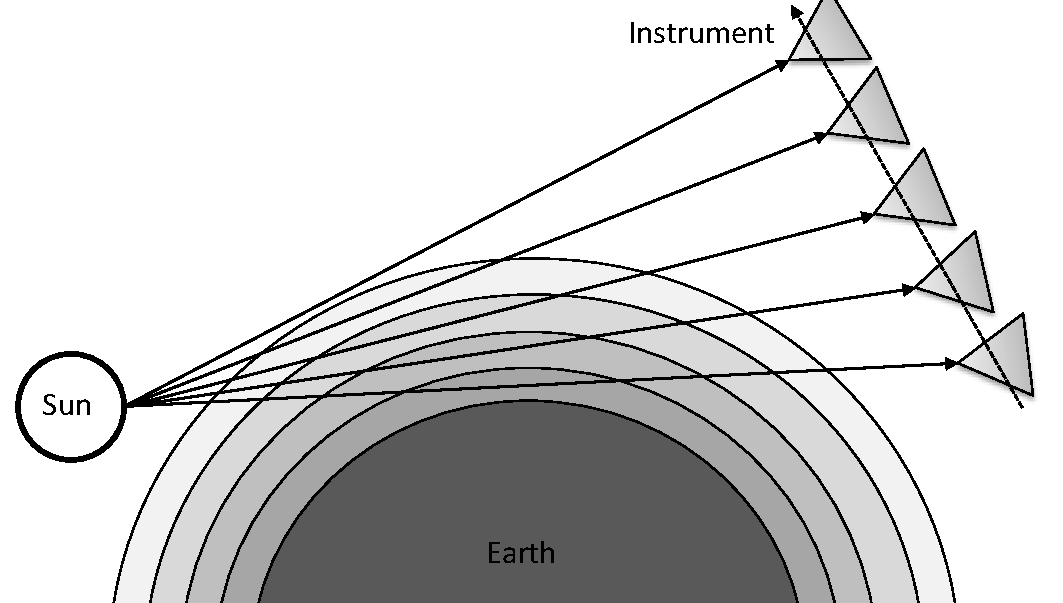
\includegraphics[width=1.0\textwidth]{./Images/OccultationGeometry.pdf}
    \caption[Occultation Geometry]{The occultation instrument monitoring the atmosphere by scanning the atmosphere by looking directly at the sun.}
    \label{fig:OccultationGeometry}
\end{figure}

\subsection{LIDAR}

Through the transmission of a laser pulse though the atmosphere, a method known as LIght Dectection and Ranging (LIDAR) can determine aerosol concentrations through the measuring of the intensity of the backscattered laser light at different wavelengths and polarizations. Initially LIDAR was primarily used at ground based facilities to measure aerosol layers dating back to the 1960s \citep{Fiocco1964}. More recently LIDAR instruments have been used on satellite missions including the Ice, Cloud, and land Elevation Satellite (ICESat) from 2002 to 2010 \citep{Schutz2005} with a second mission, ICESat-2, planed for launch in 2017 and Cloud-Aerosol Lidar and Infrared Pathfinder Satellite Observations (CALIPSO) which launched in 2006 \citep{Winker2007}. Traditional LIDAR instruments have looked in the nadir direction (straight down or up) however some instruments have looked slightly off-nadir, as seen in \autoref{fig:LidarGeometry}, to increases to signal to noise.

\begin{figure}[h]
    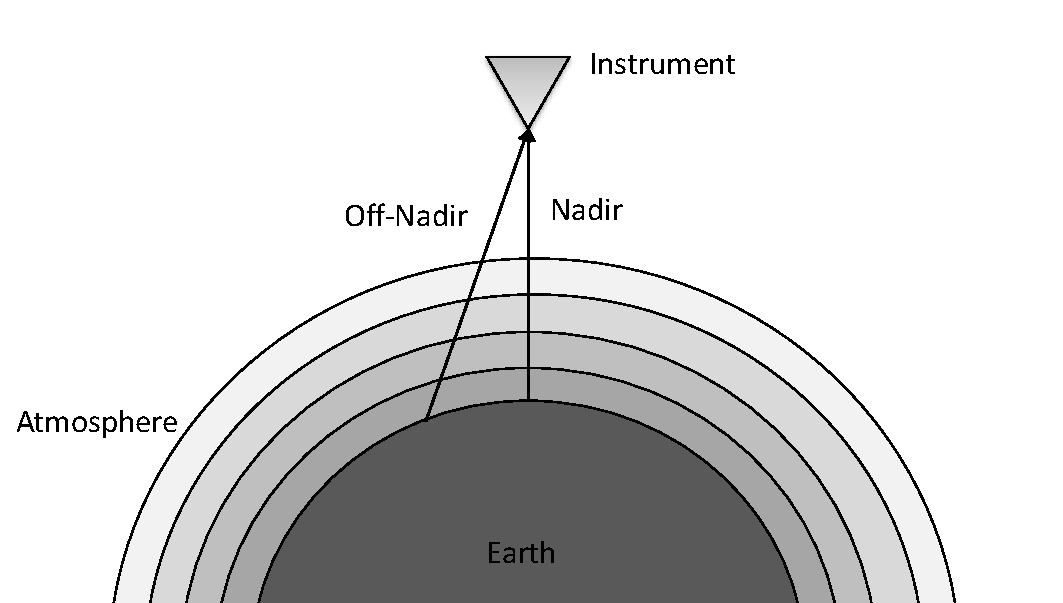
\includegraphics[width=1.0\textwidth]{./Images/LidarGeometry.pdf}
    \caption[LIDAR Geometry]{LIDAR instrument showing a measurement in both the nadir and offnadir lines of sight.}
    \label{fig:LidarGeometry}
\end{figure}

CALIPSO is a joint mission developed between the National Aeronautics and Space Administration (NASA) and the Centre National d'Etudes Spatiales (CNES) of the United States and France respectively. It uses a two wavelength polarized LIDAR system to achieve high resolution aerosol and cloud retrievals along the satellite's orbital track, it views the ground track initially at 0.3\si{\degree} off-nadir to remove specular reflection from still water and then in 2007 the angle was increased to 3\si{\degree} to reduce effects from orientated ice crystals \citep{Hu2009}. CALIPSO data is used to determine aerosol extinction profiles at 40~km horizontal resolution and 120~m vertices resolution with global coverage from 82\si{\degree}S to 82\si{\degree}N \citep{Young2009}. However, despite the excellent vertical resolution given by LIDAR satellite instruments they suffer from poor Signal to Noise Ratio (SNR) especially during the during daylight hours and for high altitude aerosol measurements \citep{Kacenelenbogen2011}.


\subsection{Limb Emission}

MIPAS and MLS (I think) now have sulphate products


\subsection{Limb Scatter}

\begin{figure}[h]
    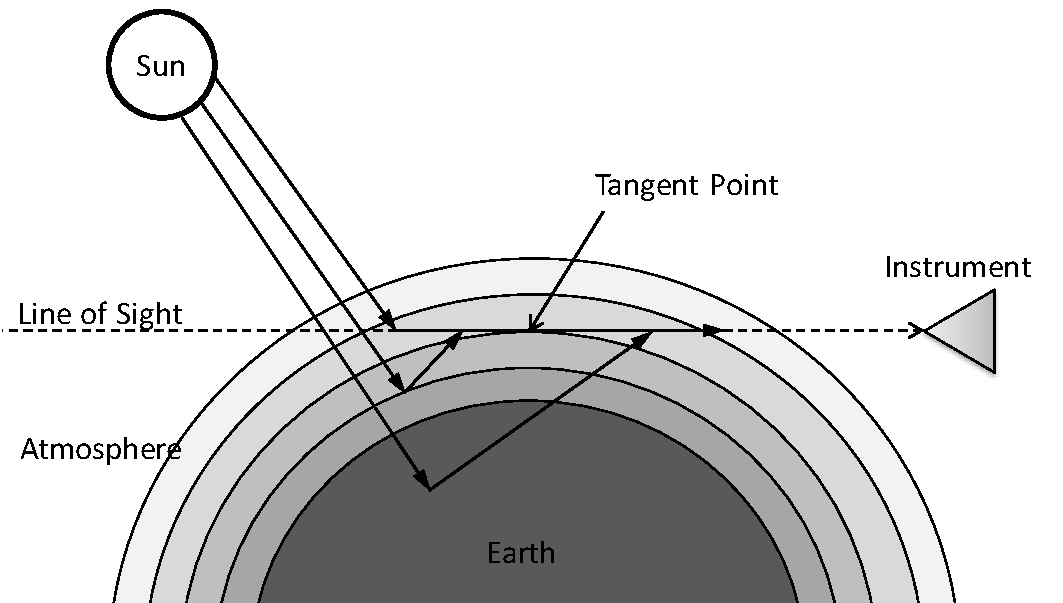
\includegraphics[width=1.0\textwidth]{./Images/LimbScatterGeometry.pdf}
    \caption[Limb Scatter Geometry]{TODO: Write this}
    \label{fig:LimbScatterGeometry}
\end{figure}

\subsubsection{Scanning}

SCIAMACHY OSIRIS

\subsubsection{Imaging}

OMPS and ALTIUS 